\section{Desarrollo}

Para el desarrollo de este trabajo se implementaron en C++ los algoritmos vistos en clase para resolver el problema de la subsecuencia de 
suma máxima, recordemos que tienen complejidades temporales distintas, las cuales son:
\begin{itemize}
    \item Algoritmo 1: Complejidad $O(n^3)$
    \item Algoritmo 2: Complejidad $O(n^2)$
    \item Algoritmo 3: Complejidad $O(n \log n)$
    \item Algoritmo 4: Complejidad $O(n)$
    \item Algoritmo 5: Complejidad $O(n)$
\end{itemize}

Una vez implementados los algoritmos, se verificó su correcto funcionamiento utilizando casos de prueba con instancias pequeñas con prubas apartir de
$n=10$ y aumentando progresivamente hasta tamaños mayores, manteniendo siempre la misma instancia de datos para todos los algoritmos 
con el fin de garantizar una comparación justa de los tiempos de ejecución. 

Se obtuvieron los siguientes resultados para cada algoritmo:

\subsection{Computadora Local (Propia)}
\begin{figure}[H]
    \centering
    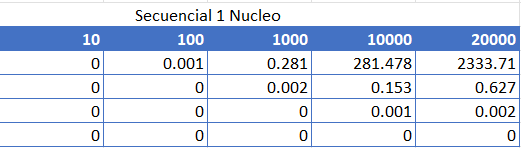
\includegraphics[width=0.5\textwidth]{rsc/img/dg_1ncl.png}
    \caption{Tiempo en segundos obtenido para cada algoritmo en computadora local.}\label{tab:dg_1ncl}
\end{figure}
\begin{figure}
    \centering
    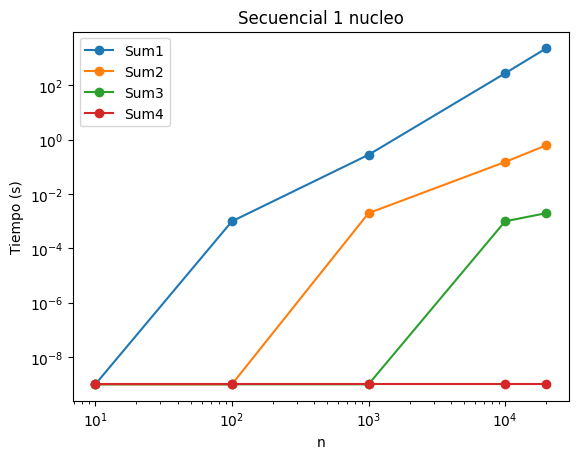
\includegraphics[width=0.5\textwidth]{rsc/img/gdg_1ncl.png}
    \caption{Grafica en escala logaritmica para cada algoritmo en computadora local.}\label{fig:gdg_1ncl}
\end{figure}

\begin{figure}[H]
    \centering
    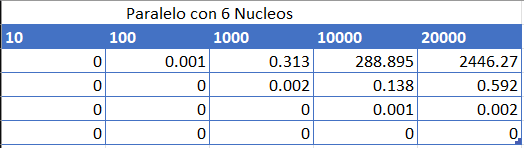
\includegraphics[width=0.5\textwidth]{rsc/img/dg_6ncl.png}
    \caption{Tiempo en segundos obtenido para cada algoritmo en computadora local.}\label{tab:dg_6ncl}
\end{figure}
\begin{figure}
    \centering
    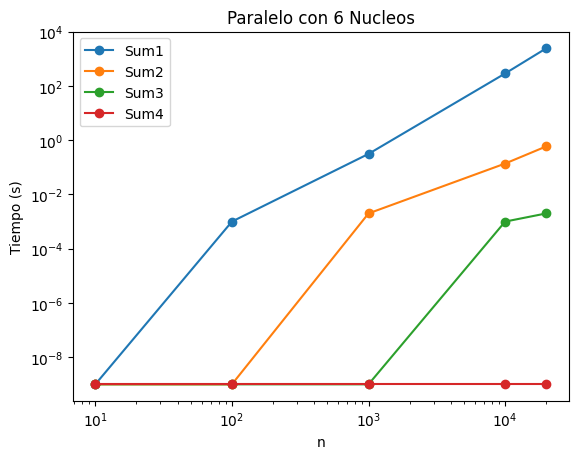
\includegraphics[width=0.5\textwidth]{rsc/img/gdg_6ncl.png}
    \caption{Grafica en escala logaritmica para cada algoritmo en computadora local.}\label{fig:gdg_6ncl}
\end{figure}

\begin{figure}[H]
    \centering
    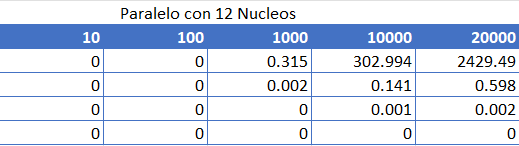
\includegraphics[width=0.5\textwidth]{rsc/img/dg_12ncl.png}
    \caption{Tiempo en segundos obtenido para cada algoritmo en computadora local.}\label{tab:dg_12ncl}
\end{figure}
\begin{figure}
    \centering
    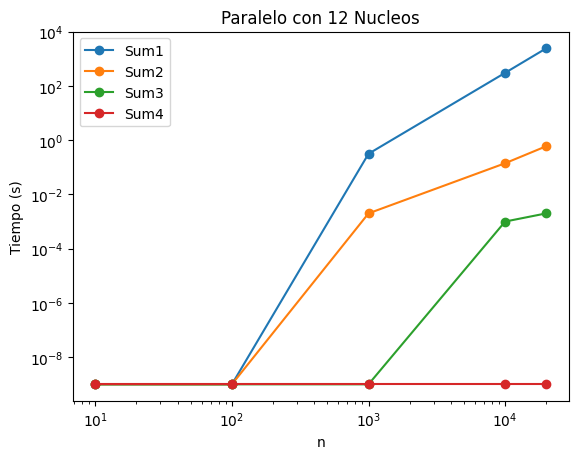
\includegraphics[width=0.5\textwidth]{rsc/img/gdg_12ncl.png}
    \caption{Grafica en escala logaritmica para cada algoritmo en computadora local.}\label{fig:gdg_12ncl}
\end{figure}

\subsection{Supercomputadora LAVIS}
\begin{figure}[H]
    \centering
    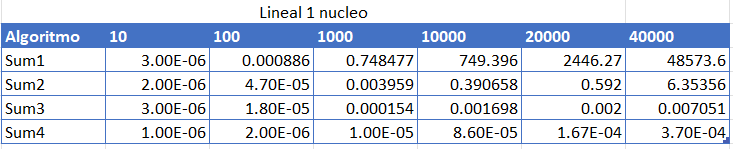
\includegraphics[width=0.5\textwidth]{rsc/img/lavis_1ncl.png}
    \caption{Tiempo en segundos obtenido para cada algoritmo en computadora local.}\label{tab:lavis_1ncl}
\end{figure}
\begin{figure}
    \centering
    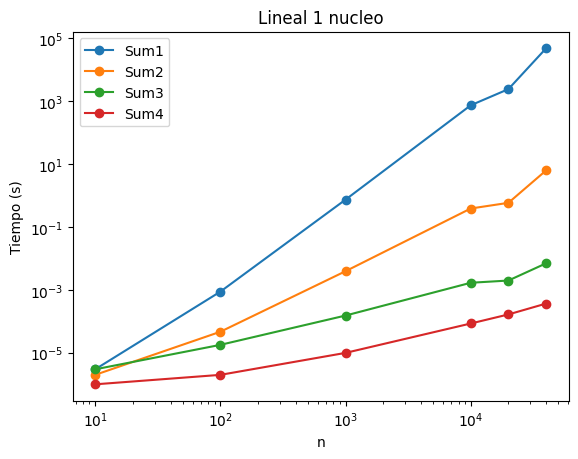
\includegraphics[width=0.5\textwidth]{rsc/img/glavis_1ncl.png}
    \caption{Grafica en escala logaritmica para cada algoritmo en computadora local.}\label{fig:glavis_1ncl}
\end{figure}

\begin{figure}[H]
    \centering
    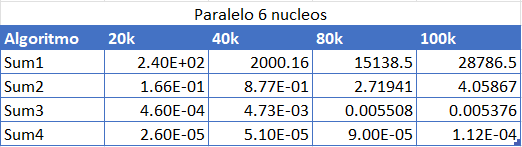
\includegraphics[width=0.5\textwidth]{rsc/img/lavis_6ncl.png}
    \caption{Tiempo en segundos obtenido para cada algoritmo en computadora local.}\label{tab:lavis_6ncl}
\end{figure}
\begin{figure}
    \centering
    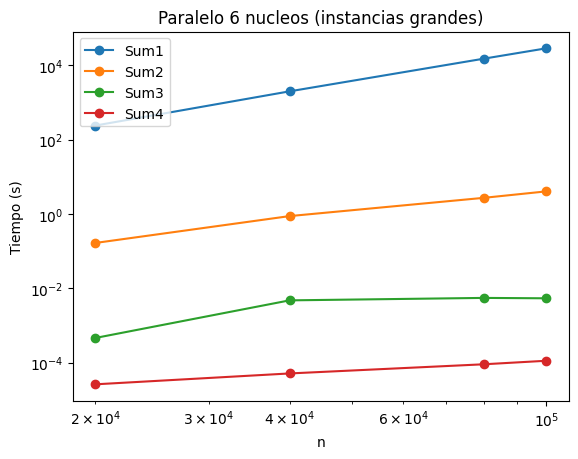
\includegraphics[width=0.5\textwidth]{rsc/img/glavis_6ncl.png}
    \caption{Grafica en escala logaritmica para cada algoritmo en computadora local.}\label{fig:glavis_6ncl}
\end{figure}

\begin{figure}[H]
    \centering
    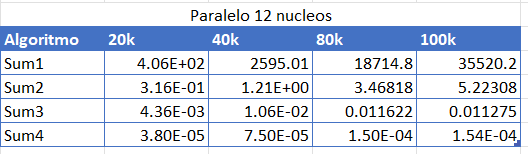
\includegraphics[width=0.5\textwidth]{rsc/img/lavis_12ncl.png}
    \caption{Tiempo en segundos obtenido para cada algoritmo en computadora local.}\label{tab:lavis_12ncl}
\end{figure}
\begin{figure}
    \centering
    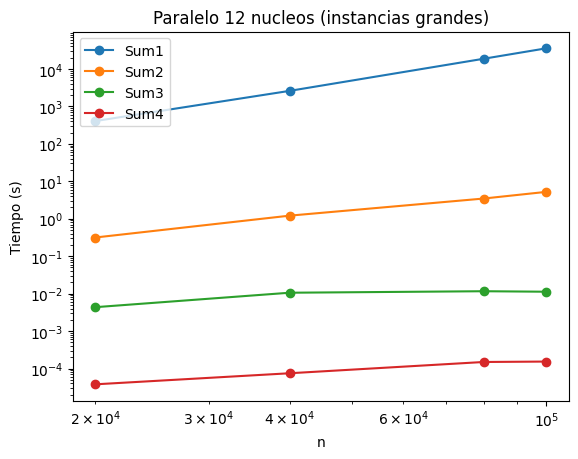
\includegraphics[width=0.5\textwidth]{rsc/img/glavis_12ncl.png}
    \caption{Grafica en escala logaritmica para cada algoritmo en computadora local.}\label{fig:glavis_12ncl}
\end{figure}

